\documentclass[english]{exam}

\setlength {\marginparwidth }{2cm} 
\usepackage{todonotes}

\usepackage[perpage,para,symbol]{footmisc}

\hyphenpenalty=15000 
\tolerance=1000

\usepackage{tikz}
\usetikzlibrary{arrows,decorations.pathmorphing,backgrounds,fit,positioning,calc,shapes}
\usepackage{pgfmath}
\usepackage{rotating}
\usepackage{array}	
\usepackage{graphicx}
\usepackage{float}	
\usepackage{mdwlist}
\usepackage{setspace}
\usepackage{listings}
\usepackage{bytefield}
\usepackage{tabularx}
\usepackage{multirow}	       
\usepackage{caption}
\usepackage{xcolor}
\usepackage{amssymb}
\captionsetup[table]{skip=10pt}

\usepackage{url}
\usepackage{hyperref}
\usepackage[all]{hypcap}	
\usepackage{titlesec}
\setcounter{secnumdepth}{4}
\titleformat{\paragraph}
{\normalfont\normalsize\bfseries}{\theparagraph}{1em}{}
\titlespacing*{\paragraph}
{0pt}{3.25ex plus 1ex minus .2ex}{1.5ex plus .2ex}

\definecolor{mGreen}{rgb}{0,0.6,0}
\definecolor{darkblue}{rgb}{0.1,0.1,0.5}
\definecolor{mGray}{rgb}{0.5,0.5,0.5}
\definecolor{mPurple}{rgb}{0.58,0,0.82}
\definecolor{backgroundColour}{rgb}{0.95,0.95,0.92}

\hypersetup{colorlinks,breaklinks,
            linkcolor=darkblue,urlcolor=darkblue,
            anchorcolor=darkblue,citecolor=darkblue}


\lstdefinestyle{CStyle}{
    backgroundcolor=\color{backgroundColour},   
    commentstyle=\color{mGreen},
    keywordstyle=\color{magenta},
    numberstyle=\tiny\color{mGray},
    stringstyle=\color{mPurple},
    basicstyle=\footnotesize,
    breakatwhitespace=false,         
    breaklines=true,                 
    captionpos=b,                    
    keepspaces=true,                 
    numbers=left,                    
    numbersep=5pt,                  
    showspaces=false,                
    showstringspaces=false,
    showtabs=false,                  
    tabsize=2,
    language=C
}

\PassOptionsToPackage{USenglish,english}{babel} 
\usepackage{csquotes}
\usepackage{tabto}
\usepackage[USenglish,english]{babel}
\usepackage[acronym, section=section, nonumberlist, nomain, nopostdot]{glossaries}
\makeglossaries
 
\makeglossaries
\newcommand{\colorbitbox}[3]{%
	\rlap{\bitbox{#2}{\color{#1}\rule{\width}{\height}}}%
	\bitbox{#2}{#3}}

\begin{document}

\title{Assignment III:\\ Advanced CUDA}
\author{Amirhossein Namazi, Calin Capitanu}

\maketitle
\begin{center}
  \url{https://github.com/capitanu/DD2360} \\
\end{center}
\chapter{Exercise 1}
\section*{CUDA Edge Detector using shared memory}

\begin{enumerate}
\item Explain how the mapping of GPU thread and thread blocks (which is already implemented for you in the code) is working. \\\\
  The thread blocks are spread into a grid, since the processing of each pixel is easier to be sent out and understood in an actual 2D format. There is a defined BLOCK\_SIZE of 16 threads (per block), and then the size of the image is divided into smaller blocks, thus creating a grid. One could easily visualize this as if pixels are grouped into small squares (the blocks) and each pixel is considered a thread inside this thread block.
  
\item Explain why shared memory can (theoretically) improve performance.\\\\
  On short, shared memory could theoretically increase the performance due to the fact that the bandwidth inside the device (GPU) is way higher than in the global memory (between CPU and GPU). However, depending on the amount of processing, it could actually not be that beneficial. If threads do not need to share much memory (for example only 1 interconnected execution), the performance could as well not be highly improved. Most of the time however, the performance is better since threads share a block of memory inside the same thread block and do not need to access the host (CPU) in order to get data from an adjacent thread.
  
\item Explain why the resulting image looks like a "grid" when the kernel is simply copying in pixels to the shared block. Explain how this is solved and what are the cases.\\\\
  Since the BLOCK\_SIZE\_SH is set with 2 more columns and 2 more rows, when the gpu\_applyFilter function is called, the whole block is sent to the function and when one arrives at the end of the block, there are these two more columns and rows that do not have any data, thus they are undefined and get unexpected results. That is due to the fact that the filter function actually does work with a 3x3 matrix, thus when arriving at the last rows and columns, there is nothing left to work with for these pixels, thus the need for extra columns and rows, in order to compute the pixel with the 3x3 filter.
  
\item There are several images of different sizes in the image folder. Try running the program on them and report how their execution time relates to file sizes.\\\\
  The short answer is yes. The images size does matter with computation time. In fact the image ``hw.bmp'' and ``nyc.bmp'' took the longest. It is also pretty intuitive that more images will take longer (unless there are enough available threads on the GPU to run all of them in parallel). ``nyc.bmp'' took around 25 ms for each run and ``hk.bmp'' took around 13-14 ms for each part, while the other took 8-9 ms. The results are displayed in the plot below.

\end{enumerate}

\clearpage
\chapter{Exercise 2}
\section*{Pinned and Managed Memory}

The results from $nvprof$ can be found in the appendix of this report.

\begin{enumerate}
\item What are the differences between pageable memory and pinned memory, what are the tradeoffs? \\\\
  The idea behind pageable memory is that the operating system tries to keep the memory pages in the physical memory as long as they are needed, but they might be moved to external storage (like hard-drives or SSDs) when they are not used anymore. The copy of data between the Host and the Device uses a hardware piece called DMA, which tries to read memory from a physical address. If that physical address in the Host is replaced (paged out), the data could be corrupt, which is the main reason of introduction of pinned memory. Pinned memory is the memory that sticks to the place where it is allocated until freed accordingly.
  
\item Do you see any difference in terms of the breakdown of execution time after changing to pinned memory from pageable memory? \\\\
  Yes, in fact results with 1000000 particles, 100 iteration and 256 block size show that the time it took with pinned memory is almost half of the time compared to when using pageable memory. This is explained mostly by the fact that the pageable memory needs to be also copied to a place with pinned memory which creates an overhead. The time for pinned memory was 0.183069, while the time for pageable memory was 0.357765.
  
\item What is a managed memory? What are the implications of using managed memory? \\\\
  Managed memory is a concept introduced together with CUDA 6. Managed memory, or unified memory is the idea of simplifcation of memory in a way where both CPU and GPU would completely share the memory. They both have access at the same time to the same block of memory that can be allocated both dynamically or statically. One implication of such managed memory for the developers is the ease of use: it simplifies the number of pointers needed, only one available both on the CPU and the GPU. The major break point is the introduction of the Pascal series of Nvidia GPUs, since they work differently. Post-Pascal GPUs may create pages and page tables only when those are accessed by either the CPU or the GPU, while pre-Pascap GPUs allocates the managed memory on the GPU.
  
\item If you are using Tegner or lab computers, the use of managed memory will result in an implicit memory copy before CUDA kernel launch. Why is that? \\\\
  Unforuntely, we are using our own Ampere GPU. However, the fact that these memory is copied to the GPU is normal, since these GPUs are pre-Pascal GPUs, and for these, before launching the kernel, the CUDA runtime will migrate all pages to the GPU memory.
\end{enumerate}

\clearpage
\chapter{Exercise 3}
\section*{CUDA Streams/Asynchronous Copy - Particle Batching}

Unfortunately, we could not get $nvvp$ to work on our local machine due to (we assume) compatibility issues (?). We think that the distribution of Linux being used is not working with this, however, the $nvprof$ logs have been added in the appendix of this document.

\begin{enumerate}
\item What are the advantages of using CUDA streams and asynchronous memory copies? \\\\
  The advantage of using CUDA streams is that we can fully utilize the GPU and all of its component. The idea is that we can have the GPU still perform computations on different kernels while also copying data to it on a different stream. That is, one stream can execute some computations while another can copy data to the device, utilizing paralellism and saving time.
  
\item What is the performance improvement (if any) in using more than one CUDA stream? \\\\
  Surprisingly enough, for the problem at hand, no major improvements were observable when adding more than one stream. We tried to understand whether or not the actual implementation of our stream process was wrong, but we hold to the fact that it is not. This is surprising to us, since again, the problem at hand seems to get worse times with more streams. However, we think that the greater the problem, the more streams could be helpful in this sense.
  
\item What is the impact of batch size on performance? \\\\
  It seems to us that the smaller the batch size, the better the performance. Once again, we think that the results are really particular to the problem at hand, and that they should not be generalized. However, the improvements are also significantly small, only showing up when the number of streams is also higher. With 128 batch size and 4 streams, our total time was 0.001302, while with the same number of streams and only 16 block size, we achieved 0.001354 ms.
\end{enumerate}

\clearpage
\chapter{Bonus Exercise}
\section*{CUDA Libraries - cuBLAS}

\begin{enumerate}
\item Explain why is the matrix size has to be a multiple of 16? \\\\
  This is because the matrix needs to be a multiple of the TILE\_SIZE. However, this can be configured in the beginning of the file, thus the matrix size could be a different number, but always a multiple of the TILE\_SIZE.
\item Refer to $shared\_sgemm\_kernel()$. There are two $\_\_syncthreads()$ in the loop. What are they used for, in the context of this code?\\\\
  There are two of these directives. The main reason for using these is the fact that this uses shared memory, and one does not want to access data that is in the process of being changed or not computed yet, but instead wants the final result before utilizing that data block, which is the case with the two tiles. If one operates multiple times on a piece of data asynchronously, one could get corrupted data. Using mutexes is not needed for this, however, waiting for all the processes is needed in order to continue.
  \begin{enumerate}
  \item What is the directive that can potentially improve performance in the actual multiplication? What does it do?\\\\
    The directive we used is $\#pragme unroll$. This directive tries to optimize a loop in the sense that instead of it running a specified number of times, all the specific lines in the loop are placed in the code. In our case, most probably, all of the second part of the additions are calculated at once and added to the variable $val$. This eliminates the checks for $k < TILE\_SIZE$ and all of the assignment of values to $k$ and so on.
  \item There is a large speedup after switching from using global memory to shared memory, compared to the Edge Detector in Exercise 1. What might be the reason?\\\\
    We assume that in this case, the speedup is due to the amount of operations that are being done in a single thread. That is, in the edge computation we only applied two filters (low number of computation) on each pixel, but in this case, we run a loop of operations and a lot more accesses to the memory, which in this case is really valuable.
  \end{enumerate}
\item Refer to $cublas\_sgemm$. We asked that you compute $C=BA$ instead of $C=AB$.
  \begin{itemize}
  \item It has to do with an important characteristic of how to use cuBLAS. What is that, and why do we do C=BA? \\\\
    The library cuBLAS is based on the original BLAS library that was written in FORTRAN. This library uses ``column-major'' array storage, which means that, basically, the first index when addressing a 2D array is the column instead of the row. Again, cuBLAS is configured in the same way. This means that the memory layout of these is also reversed, which means items in the same column are placed closer to each-other, instead of previously with the row neighbours being actually located closer in the memory address. Again, this is just an assumption, but we assume that by doing $BA$ instead of $AB$, the spatial locality is being used better. We could be completely wrong about the spatial locality here, but this multiplication is definitely done this way due to the column-major architecture of 2D arrays that this library uses.
  \end{itemize}
\item Run the program with different input sizes, for example from 64, 128, ..., to 4096.
  \begin{itemize}
  \item Make a grouped bar plot of the execution times of the different versions (CPU, GPU Global, GPU Shared, GPU cuBLAS). You can plot CPU results in a separate figure if the execution time goes out of the scale compared to the rest. \\\\

    The plots are displayed below, however I want to mention that the second plot is similar to the first one, only that the last result has been scaled down in order to make all of the other results visible. The results specifically are also listed before the plots:
    \lstset{
      basicstyle=\fontsize{6}{8}\selectfont\ttfamily
    }

    \begin{lstlisting}
cpu = [0.751000, 5.815000, 47.443000, 368.392000, 2968.284000, 23683.770000, 191485.124000]
cublas = [0.205000, 0.270000, 0.310000, 0.223000, 0.400000, 0.998000, 6.396000]
gpu_global = [0.015000, 0.021000, 0.086000, 0.612000, 4.928000, 38.110000, 23.464000]
gpu_shared = [0.009000, 0.010000, 0.023000, 0.118000, 0.830000, 7.281000, 52.357000]
    \end{lstlisting}
  \end{itemize}
\begin{center}
    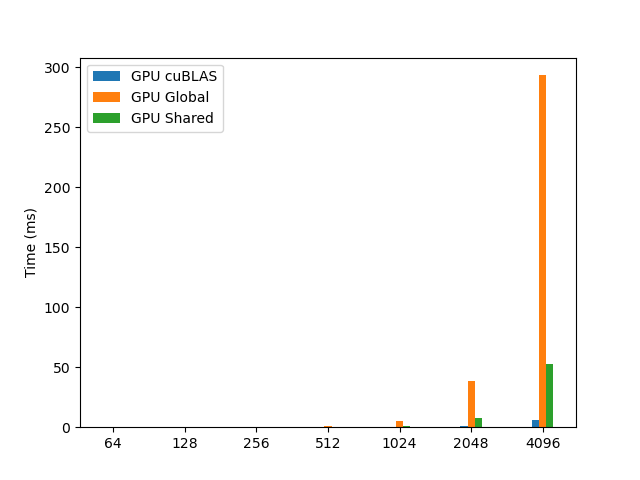
\includegraphics[scale=0.65]{gpu1.png}
  \end{center}

  \begin{center}
    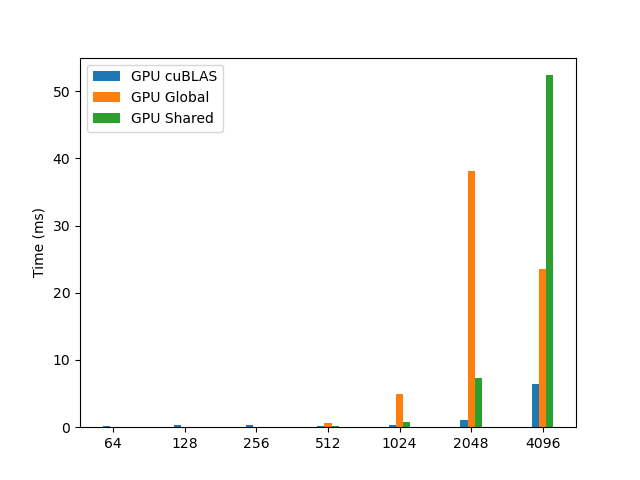
\includegraphics[scale=0.65]{gpu2.png}
  \end{center}

  \begin{center}
    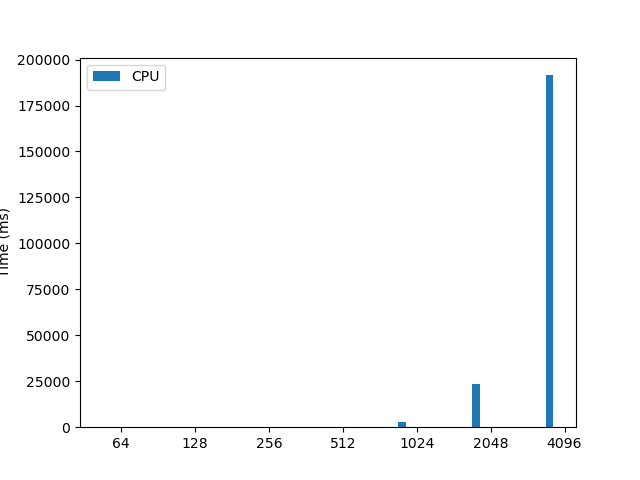
\includegraphics[scale=0.65]{gpu3.png}
  \end{center}

  
\end{enumerate}

\clearpage
\chapter{Appendix}
\section*{Exercise 2 - nvprof (nsys)}

\lstset{
  basicstyle=\fontsize{6}{8}\selectfont\ttfamily
}

\subsection*{All particles copied at the beginning of a time step}

\begin{lstlisting}
  CUDA API Statistics:

 Time (%)  Total Time (ns)  Num Calls    Avg (ns)       Med (ns)      Min (ns)     Max (ns)    StdDev (ns)          Name         
 --------  ---------------  ---------  -------------  -------------  -----------  -----------  -----------  ---------------------
     76.1      341,458,476        200    1,707,292.4    1,758,252.0    1,471,761    6,888,887    407,013.4  cudaMemcpy           
     23.8      106,628,402          1  106,628,402.0  106,628,402.0  106,628,402  106,628,402          0.0  cudaMalloc           
      0.1          537,211        100        5,372.1        4,810.0        3,880       19,460      1,953.8  cudaLaunchKernel     
      0.0          139,370        100        1,393.7        1,250.0          950        3,450        362.4  cudaDeviceSynchronize
      0.0          120,491          1      120,491.0      120,491.0      120,491      120,491          0.0  cudaFree             

[5/7] Executing 'gpukernsum' stats report

CUDA Kernel Statistics:

 Time (%)  Total Time (ns)  Instances  Avg (ns)  Med (ns)  Min (ns)  Max (ns)  StdDev (ns)                 Name                
 --------  ---------------  ---------  --------  --------  --------  --------  -----------  -----------------------------------
    100.0        9,177,266        100  91,772.7  91,614.0    89,022   124,989      3,529.4  timestepKernel(Particle *, double3)

[6/7] Executing 'gpumemtimesum' stats report

CUDA Memory Operation Statistics (by time):

 Time (%)  Total Time (ns)  Count   Avg (ns)     Med (ns)    Min (ns)   Max (ns)   StdDev (ns)      Operation     
 --------  ---------------  -----  -----------  -----------  ---------  ---------  -----------  ------------------
     51.8      164,055,870    100  1,640,558.7  1,573,324.0  1,535,006  6,239,379    469,419.6  [CUDA memcpy DtoH]
     48.2      152,614,204    100  1,526,142.0  1,494,142.0  1,455,359  2,421,577    122,948.6  [CUDA memcpy HtoD]

[7/7] Executing 'gpumemsizesum' stats report

CUDA Memory Operation Statistics (by size):

 Total (MB)  Count  Avg (MB)  Med (MB)  Min (MB)  Max (MB)  StdDev (MB)      Operation     
 ----------  -----  --------  --------  --------  --------  -----------  ------------------
  2,400.000    100    24.000    24.000    24.000    24.000        0.000  [CUDA memcpy DtoH]
  2,400.000    100    24.000    24.000    24.000    24.000        0.000  [CUDA memcpy HtoD]

\end{lstlisting}

\subsection*{All particles copied at the beginning of a time step - cudaMallocHost}

\begin{lstlisting}
  CUDA API Statistics:

 Time (%)  Total Time (ns)  Num Calls    Avg (ns)       Med (ns)      Min (ns)     Max (ns)    StdDev (ns)           Name         
 --------  ---------------  ---------  -------------  -------------  -----------  -----------  ------------  ---------------------
     64.5      182,693,127        200      913,465.6          290.0          270  179,917,363  12,722,538.4  cudaMemcpy           
     35.5      100,564,470          1  100,564,470.0  100,564,470.0  100,564,470  100,564,470           0.0  cudaHostAlloc        
      0.0           51,290        100          512.9          290.0          280       17,090       1,706.9  cudaLaunchKernel     
      0.0           36,140        100          361.4          300.0          290        2,550         238.8  cudaDeviceSynchronize
      0.0            1,130          1        1,130.0        1,130.0        1,130        1,130           0.0  cudaFree             

[5/7] Executing 'gpukernsum' stats report
SKIPPED: /home/calin/kth/TCSCM1/DD2360_Applied_GPU_Programming/assignments/Assignment_3/ex_2/my_report.sqlite
does not contain CUDA kernel data.
[6/7] Executing 'gpumemtimesum' stats report
SKIPPED: /home/calin/kth/TCSCM1/DD2360_Applied_GPU_Programming/assignments/Assignment_3/ex_2/my_report.sqlite
does not contain GPU memory data.
[7/7] Executing 'gpumemsizesum' stats report
SKIPPED: /home/calin/kth/TCSCM1/DD2360_Applied_GPU_Programming/assignments/Assignment_3/ex_2/my_report.sqlite
does not contain GPU memory data.

\end{lstlisting}
\clearpage
\subsection*{Managed Memory}

\begin{lstlisting}
  CUDA API Statistics:

 Time (%)  Total Time (ns)  Num Calls    Avg (ns)       Med (ns)      Min (ns)     Max (ns)    StdDev (ns)          Name         
 --------  ---------------  ---------  -------------  -------------  -----------  -----------  -----------  ---------------------
     89.1      110,713,636          1  110,713,636.0  110,713,636.0  110,713,636  110,713,636          0.0  cudaMallocManaged    
     10.9       13,484,590        100      134,845.9          280.0          270   13,453,500  1,345,318.6  cudaDeviceSynchronize
      0.0           56,840        100          568.4          260.0          250       27,280      2,701.0  cudaLaunchKernel     
      0.0              990          1          990.0          990.0          990          990          0.0  cudaFree             

[5/7] Executing 'gpukernsum' stats report
SKIPPED: /home/calin/kth/TCSCM1/DD2360_Applied_GPU_Programming/assignments/Assignment_3/ex_2/my_report.sqlite does not contain
CUDA kernel data.
[6/7] Executing 'gpumemtimesum' stats report

CUDA Memory Operation Statistics (by time):

 Time (%)  Total Time (ns)  Count  Avg (ns)  Med (ns)  Min (ns)  Max (ns)  StdDev (ns)              Operation            
 --------  ---------------  -----  --------  --------  --------  --------  -----------  ---------------------------------
    100.0        2,999,937    962   3,118.4   1,983.0     1,503    70,463      5,082.9  [CUDA Unified Memory memcpy HtoD]

[7/7] Executing 'gpumemsizesum' stats report

CUDA Memory Operation Statistics (by size):

 Total (MB)  Count  Avg (MB)  Med (MB)  Min (MB)  Max (MB)  StdDev (MB)              Operation            
 ----------  -----  --------  --------  --------  --------  -----------  ---------------------------------
     24.003    962     0.025     0.008     0.004     0.954        0.076  [CUDA Unified Memory memcpy HtoD]

\end{lstlisting}

\subsection*{Cuda Stream - 1 stream}

\begin{lstlisting}
CUDA API Statistics:

 Time (%)  Total Time (ns)  Num Calls    Avg (ns)     Med (ns)    Min (ns)    Max (ns)   StdDev (ns)         Name       
 --------  ---------------  ---------  ------------  -----------  ---------  ----------  ------------  -----------------
     90.3       94,922,615          4  23,730,653.8      1,645.0      1,160  94,918,165  47,458,340.8  cudaStreamCreate 
      8.9        9,349,946          1   9,349,946.0  9,349,946.0  9,349,946   9,349,946           0.0  cudaFree         
      0.4          402,210        100       4,022.1      3,835.0      3,610      14,370       1,094.1  cudaMemcpyAsync  
      0.3          312,151        100       3,121.5      2,875.0      2,730      15,440       1,354.6  cudaLaunchKernel 
      0.1          100,561          1     100,561.0    100,561.0    100,561     100,561           0.0  cudaMalloc       
      0.0            6,990          4       1,747.5      1,100.0        990       3,800       1,370.2  cudaStreamDestroy

[5/7] Executing 'gpukernsum' stats report

CUDA Kernel Statistics:

 Time (%)  Total Time (ns)  Instances  Avg (ns)  Med (ns)  Min (ns)  Max (ns)  StdDev (ns)                 Name                
 --------  ---------------  ---------  --------  --------  --------  --------  -----------  -----------------------------------
    100.0        9,516,176        100  95,161.8  91,790.0    90,622   378,072     28,912.8  timestepKernel(Particle *, double3)

[6/7] Executing 'gpumemtimesum' stats report

CUDA Memory Operation Statistics (by time):

 Time (%)  Total Time (ns)  Count  Avg (ns)  Med (ns)  Min (ns)  Max (ns)  StdDev (ns)      Operation     
 --------  ---------------  -----  --------  --------  --------  --------  -----------  ------------------
    100.0          262,844    100   2,628.4   2,528.0     2,144     4,032        380.9  [CUDA memcpy HtoD]

[7/7] Executing 'gpumemsizesum' stats report

CUDA Memory Operation Statistics (by size):

 Total (MB)  Count  Avg (MB)  Med (MB)  Min (MB)  Max (MB)  StdDev (MB)      Operation     
 ----------  -----  --------  --------  --------  --------  -----------  ------------------
      2.458    100     0.025     0.025     0.025     0.025        0.000  [CUDA memcpy HtoD]  
\end{lstlisting}

\subsection*{Cuda Stream - 2 stream}

\begin{lstlisting}
CUDA API Statistics:

 Time (%)  Total Time (ns)  Num Calls    Avg (ns)      Med (ns)     Min (ns)    Max (ns)   StdDev (ns)         Name       
 --------  ---------------  ---------  ------------  ------------  ----------  ----------  ------------  -----------------
     83.2       96,267,787          4  24,066,946.8       1,685.0       1,240  96,263,177  48,130,820.2  cudaStreamCreate 
     15.4       17,840,100          1  17,840,100.0  17,840,100.0  17,840,100  17,840,100           0.0  cudaFree         
      0.7          822,731        200       4,113.7       3,860.0       3,600      24,280       1,638.3  cudaMemcpyAsync  
      0.5          603,702        200       3,018.5       2,890.0       2,740      17,200       1,046.8  cudaLaunchKernel 
      0.1          103,810          1     103,810.0     103,810.0     103,810     103,810           0.0  cudaMalloc       
      0.0            6,700          4       1,675.0       1,065.0         920       3,650       1,320.3  cudaStreamDestroy

[5/7] Executing 'gpukernsum' stats report

CUDA Kernel Statistics:

 Time (%)  Total Time (ns)  Instances  Avg (ns)   Med (ns)   Min (ns)  Max (ns)  StdDev (ns)                 Name                
 --------  ---------------  ---------  ---------  ---------  --------  --------  -----------  -----------------------------------
    100.0       22,267,350        200  111,336.8  106,957.5    97,022   379,512     31,398.3  timestepKernel(Particle *, double3)

[6/7] Executing 'gpumemtimesum' stats report

CUDA Memory Operation Statistics (by time):

 Time (%)  Total Time (ns)  Count  Avg (ns)  Med (ns)  Min (ns)  Max (ns)  StdDev (ns)      Operation     
 --------  ---------------  -----  --------  --------  --------  --------  -----------  ------------------
    100.0          553,141    200   2,765.7   2,719.5     2,208     4,960        378.1  [CUDA memcpy HtoD]

[7/7] Executing 'gpumemsizesum' stats report

CUDA Memory Operation Statistics (by size):

 Total (MB)  Count  Avg (MB)  Med (MB)  Min (MB)  Max (MB)  StdDev (MB)      Operation     
 ----------  -----  --------  --------  --------  --------  -----------  ------------------
      4.915    200     0.025     0.025     0.025     0.025        0.000  [CUDA memcpy HtoD]  
\end{lstlisting}

\subsection*{Cuda Stream - 4 stream}

\begin{lstlisting}
CUDA API Statistics:

 Time (%)  Total Time (ns)  Num Calls    Avg (ns)      Med (ns)     Min (ns)    Max (ns)  
 StdDev (ns)         Name       
 --------  ---------------  ---------  ------------  ------------  ----------  ---------- 
 ------------  -----------------
     70.5       93,012,791          4  23,253,197.8       1,520.0       1,090  93,008,661 
 46,503,642.2  cudaStreamCreate 
     27.3       36,058,133          1  36,058,133.0  36,058,133.0  36,058,133  36,058,133 
          0.0  cudaFree         
      1.2        1,592,242        400       3,980.6       3,840.0       3,370      13,320 
        689.3  cudaMemcpyAsync  
      0.9        1,154,013        400       2,885.0       2,820.0       2,490      16,840 
        746.9  cudaLaunchKernel 
      0.1          104,540          1     104,540.0     104,540.0     104,540     104,540 
          0.0  cudaMalloc       
      0.0            7,090          4       1,772.5       1,125.0       1,000       3,840 
      1,382.8  cudaStreamDestroy

[5/7] Executing 'gpukernsum' stats report

CUDA Kernel Statistics:

 Time (%)  Total Time (ns)  Instances  Avg (ns)   Med (ns)   Min (ns)  Max (ns)  StdDev (ns)                 Name                
 --------  ---------------  ---------  ---------  ---------  --------  --------  -----------  -----------------------------------
    100.0       45,217,580        400  113,044.0  107,102.0    99,422   630,802     42,445.6  timestepKernel(Particle *, double3)

[6/7] Executing 'gpumemtimesum' stats report

CUDA Memory Operation Statistics (by time):

 Time (%)  Total Time (ns)  Count  Avg (ns)  Med (ns)  Min (ns)  Max (ns)  StdDev (ns)      Operation     
 --------  ---------------  -----  --------  --------  --------  --------  -----------  ------------------
    100.0        1,081,151    400   2,702.9   2,624.0     2,080     6,368        374.5  [CUDA memcpy HtoD]

[7/7] Executing 'gpumemsizesum' stats report

CUDA Memory Operation Statistics (by size):

 Total (MB)  Count  Avg (MB)  Med (MB)  Min (MB)  Max (MB)  StdDev (MB)      Operation     
 ----------  -----  --------  --------  --------  --------  -----------  ------------------
      9.830    400     0.025     0.025     0.025     0.025        0.000  [CUDA memcpy HtoD]
  
\end{lstlisting}

\bibliographystyle{myIEEEtran}
\renewcommand{\bibname}{References}
\addcontentsline{toc}{chapter}{References}
\bibliography{references}

\end{document}
